\section*{Aufgabe 7}

Es sei $G$ die Menge aller Geraden in der euklidischen Ebene.\\
Prüfen Sie, ob die folgenden Relationen $P$ und $S$ in $G \times G$ Äquivalenzrelationen sind:\\

a) $g_1 P g_2 \Leftrightarrow g_1 \text{ ist parallel zu } g_2$\\

\textit{Eine Äquivalenzrelation hat die Eigenschaften Reflexivität, Symmetrie und Trasitivität.}\\

\textit{Reflixiv:}\\
\textit{$g_1Pg_1$. Jede Gerade ist parallel zu sich selbst. Somit ist es reflexiv.}\\

\textit{Symmetrie:}\\
\textit{$g_1Pg_2 \Leftarrow g_2Pg_1$. Ist eine Gerade $g_1$ parallel zu einer Gerade $g_2$ folgt daraus, dass $g_2$ auch parallel zu $g_1$ ist. Somit ist es symmetrisch.}\\

\textit{Transitiv:}\\
\textit{$g_1Pg_2 \land g_2Pg_3 \Rightarrow g_1Pg_3$. Ist eine Gerade $g_1$ parallel zu einer Gerade $g_2$ und ist Gerade $g_2$ parallel zu $g_3$, so ist $g_1$ auch parallel zu $g_3$. Somit ist die transitiv.}\\

\textit{Da alle drei Eigenschaften zutreffen, handelt es sich bei $P$ um eine Äquivalenzrelation.}

\begin{figure}[h]
\centering
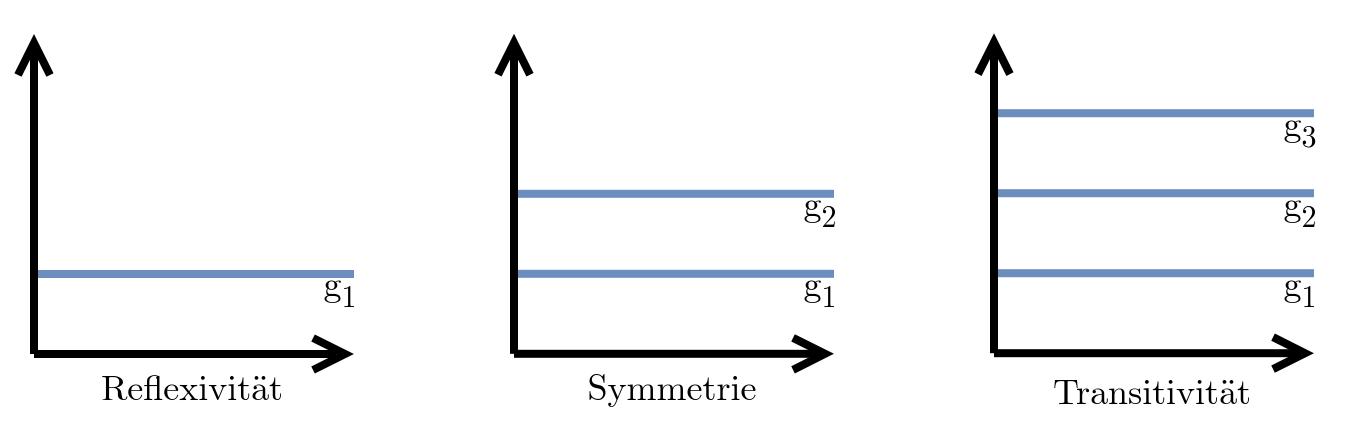
\includegraphics[width=0.8\textwidth]{graphics/parallel.png}
\end{figure}

b) $g_1 S g_2 \Leftrightarrow g_1 \text{ ist senkrecht zu } g_2$\\

\textit{Eine Äquivalenzrelation hat die Eigenschaften Reflexivität, Symmetrie und Trasitivität.}\\

\textit{Reflixiv:}\\
\textit{$g_1Sg_1$. Eine Gerade kann nicht senkrecht zu sich selbst stehen. Somit ist es nicht reflexiv.}\\

\textit{Es handelt es sich bei $S$ um keine Äquivalenzrelation.}
